% !TEX root = ../rasd.tex
\chapter{Functional Requirements and Scenarios}

% Parte da copiare all'inizio di ogni capitolo
\setmyfancystyle
% ----------------

\label{reqs}
This chapter presents the functional requirements of the system, already introduced in the previous chapter functionalities. At the beginning they will be presented in natural language as scenarios, then from these scenarios a higher level description will be abstracted. This last section will present the use-cases in the form of UML and sequence diagrams.

\section{Scenarios Natural Language Description}
As an example, the story of the \gls{passenger} Albert and the taxi \gls{driver} Bob is shown.

\subsection{System Registration}
Albert is new in the system and wants to register. He clicks on the "Register" button and he's redirected on the registration page. He inserts his personal information, like name and surname, gender, birthday, city of residence, personal tax code, e-mail and passwords. Then he submits the request to the system. The data sent are checked by the system to prevent hacks and to ensure that Albert with that personal tax code is not already registered. If the registration is successful a confirmation link is sent to the e-mail address specified by Albert and he's redirected to a login page, otherwise an error message is displayed.\\
Instead, Bob doesn't need to register itself to the system, because the cab company automatically inserts his on the system and then gives his the access keys. Besides, no confirmation is required for a taxi \gls{driver}, so no messages are sent to Bob.

\subsection{Log in}
Albert is already registered and wants to log in. He clicks on the login button and he's asked to insert his own e-mail address and password. If the combination of data is correct but he hasn't clicked yet on the confirmation link sent to his e-mail address, the login is refused and a message is shown that reminds him to do it. If the combination of data is correct and Albert has already confirmed the e-mail address he can enter the system. Otherwise if the combination isn't correct an error message appears.

\subsection{Manage personal information} 
Once Albert is logged into the system, he wants to manage his personal information, like changing the e-mail address (if he does it he has to confirm again the new address by clicking the link received in a new e-mail), city of residence, or adding other optional data, like his occupation, ...

\subsection{Management of work shifts}
Bob is already a registered \gls{driver} in the system and wants to manage his work shifts. He clicks the corresponding button on his profile page, then a form is shown with all the week days and for each day an input field for the starting hour and an input field for the ending hour of his work shift. Bob has to select which days of the week he works and the hours. Finally he submits the information.

\subsection{Start waiting time}
Bob today starts to work now and has to notify the system that he is available. He clicks the corresponding button on his profile page to start the waiting time, then a \gls{map} is shown in his \gls{ma} with his current position given by the \gls{gps} and the current address is written and can be manually modified. If the \gls{gps} is not working Bob has to manually specify his position by inserting the address and has to submit the information.\\
Therefore the ride's allocator inserts Bob in the queue of availables \gls{driver} for the city area where he is.

\subsection{Ask for a zerotime ride}
Now that Albert has entered the system he can have access to all the features available to a \gls{passenger}. He wants to ask for a zerotime ride and clicks the corresponding button in his user profile page. A \gls{map} is shown with the current position obtained by the \gls{gps} of the \gls{ma} of Albert and the actual address is written and can be manually modified by the user. If the \gls{gps} is not working or Albert is accessing the service via the WS, a message is shown claiming that the current position cannot be found and Albert has to manually specify the address of his actual position.\\
Albert submits his actual position and then he has to specify also his destination by selecting a point in the next \gls{map} that is shown or by writing the destination address in the corresponding text field.\\
The current position and the destination address are verified, if they are correct the travelling information are shown to Albert, like the estimated travelling time for the ride and the price. Albert must finally confirm the ride request. Instead if the starting or the destination addresses are invalid an error message is displayed and Albert has to correct them.\\
\\
After Albert's final confirmation, the ride's allocator contacts the first available \gls{driver} in the queue near Albert's position.\\
Bob is the first available \gls{driver} near Albert's position and receives a notification through the \gls{ma} on his smartphone. He is asked to choose whether to accept the ride or to reject it. If he declines it another \gls{driver} in the queue will be notified.\\
Bob accepts the ride.\\
\\
After Bob's confirmation the ride's allocator remove Bob from the queue of available \glspl{driver}, calculates the estimated time and sends a notification to Albert with the estimated waiting time, the \gls{driver}'s name and his cab car-code, through his \gls{ma} and e-mail.\\
\\
Today Bob is waiting for a ride in front of the railway station. Albert, who was arrived in the city by train a few minutes ago, sees the parked taxi and asks him a ride. Bob uses the same functionality shown above to notifies the system that he is no longer available for the rides.

\subsection{End of a ride}
Albert has reached his destination and pays Bob for the ride. Bob now has to notify the system that he is available again. He clicks the start waiting time button in his profile page, then a \gls{map} is shown in his \gls{ma} with his current position given by the \gls{gps} and the current address is written and can be manually modified. If the \gls{gps} is not working Bob has to manually specify his position by inserting the address and has to submit the information.\\
Therefore the ride allocator inserts again Bob in the queue of available \glspl{driver} for the city area where he is now.

\subsection{Book a future ride}
Albert wants to book a \gls{future} ride for a week later, he clicks the corresponding button in his user profile page. Albert is asked to select the date for the ride that can be only between 30 days later and the starting position by selecting a point in the \gls{map} that is shown or by manually writing the address in the corresponding text field. He submits the information and then he has to specify the destination position in the same way of the starting position and has to submit it.\\
The starting and destination position are verified, if they are correct the travelling information are shown to Albert, like the estimated travelling time for the ride and the price. Instead if the starting or the destination position are invalid an error message is displayed and Albert has to correct them. Albert must finally confirm the ride request. 
After the confirmation the ride \gls{reservation} is saved and Albert can view it (with all the information), modify it or cancel it, by accessing to his \glspl{reservation} page by clicking the corresponding button in his profile page.\\
Albert might change idea and delete his ride booking during the next seven days until 15 minutes before the chosen ride time.\\
\\
After seven days, 1 hour before the chosen ride time Albert receives a reminder of his booking via the \gls{ma} and the e-mail.\\
Albert hasn't cancelled his \gls{reservation}, so 10 minutes before the chosen time, the system starts all the operations described before to contact an available \gls{driver} and assign him to the Albert's ride.

\subsection{Check the reservations}
Albert wants to check his \glspl{reservation} and clicks the corresponding button in his user profile page. A list of all the \glspl{reservation} (also the zero-time rides) ever made by Albert are shown, with all the information, divided per page and in descending order by date. The \gls{future} rides not yet completed have a button beside to modify the date or to cancel them. If Albert clicks the modify button he's redirected to the same page of the \gls{future} ride booking.

\subsection{Read the alerts}
Albert wants to read his received \glspl{alert} and clicks the corresponding button in his user profile page. A list of all the \glspl{alert}/notifications he has ever received is shown, with all the information, divided per page and in descending order by date.



\section{Functional Requirements Scheme Description}
In this paragraph are shown all the functionalities in a formal way, using Sequence Diagrams, UML modeling and flow sequences with related actors, preconditions, postconditions and exceptions.\\
\\
An important note is the following: if an input error is modelled in a sequence diagram, it is usually represented as an alternative frame. Hence, when the input data are received and checked by the system, there are two alternatives: the data are correct, thus the operations follows the right sequence; the data are incorrect and an error message is shown. We made this choice due to simplify all the sequence diagrams: obviously any control on the inserted data is repeated in a loop until they are acceptable.


\subsection{Use Case Diagram}
The \figurename~\ref{ucDia} gives an overview on the main actors involved in the system and the functionalities that they are able to execute.

\begin{figure}
	\centerline{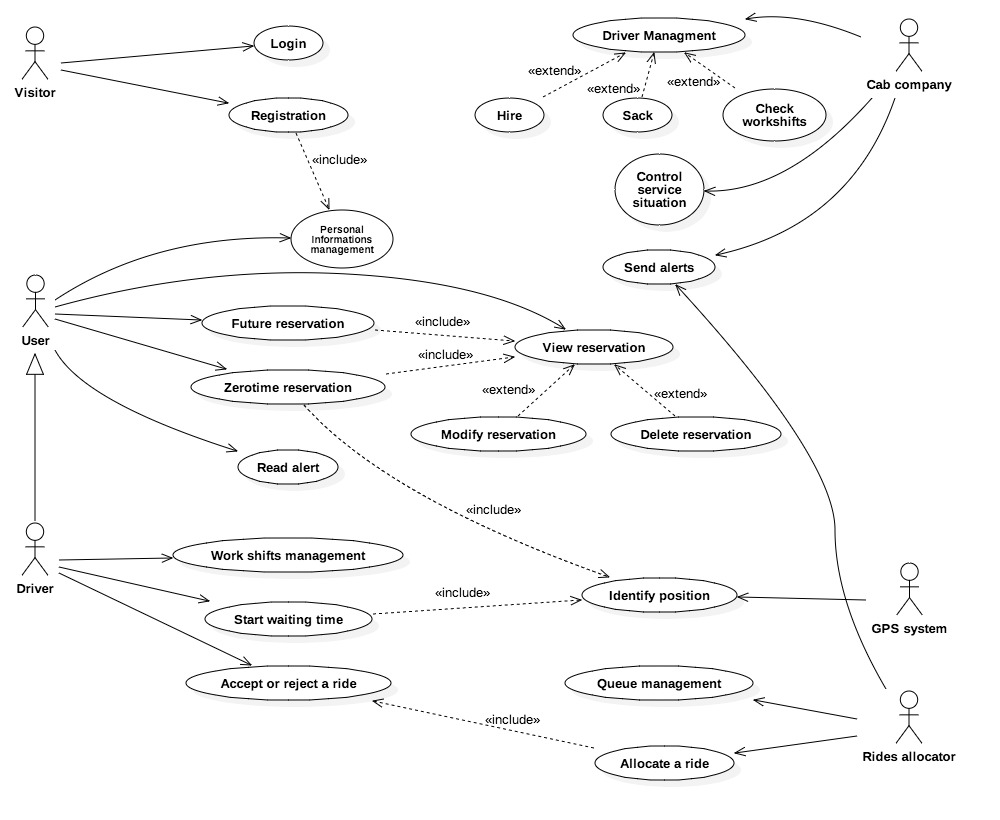
\includegraphics[width=\paperwidth]{./figures/UseCaseDiagram.jpg}}
	\caption{Use Case Diagram for myTaxiService}
	\label{ucDia}
\end{figure}

\clearpage

\subsection{UML Class Diagram}
The \figurename~\ref{cDia} describes a first proposal of entities and their relation.\\
\\

\begin{figure}[h!]
	\centerline{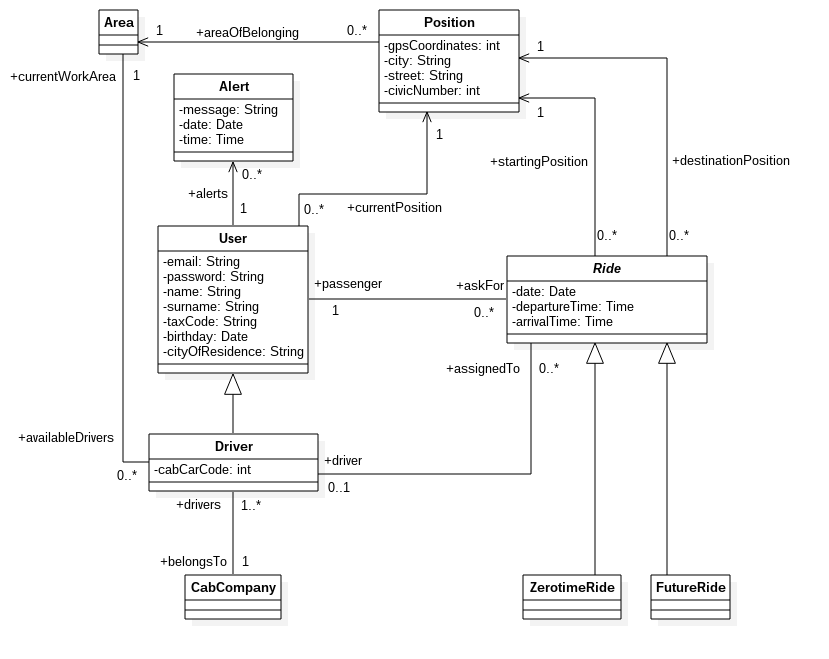
\includegraphics[width=\textwidth]{./figures/ClassDiagram.png}}
	\caption{Class diagram for myTaxyService}
	\label{cDia}
\end{figure}

\clearpage

\subsection{Registration}
\begin{tabular}{lp{8cm}}
	\hline 
	Actors & Visitor  \\ \hline
	Preconditions & The visitor has never registered before in the system.  \\ \hline
	Execution Flow &  \begin{enumerate}
					\item The visitor accesses the registration page.
					\item The system asks the visitor to insert personal informations: name, surname, gender, address, date of birth, email, tax code, and a password used to access the myTaxiService from now.
					\item The system checks the data, the tax code's unicity and the correctness of the email address.
					\item The system sends the confirmation link by email and notifies the correct registration.
					\item The visitor clicks on the confirmation link.
					\item The system redirects the visitor to the login page.
				\end{enumerate}
	 \\ \hline
	 Postconditions & The Visitor is now registered on the system, but it isn't logged in yet. \\ \hline
	 Exceptions &  The tax code already exists in the system (so the visitor is already registered), the inserted email is nonexistent or invalid, the visitor doesn't complete the registration clicking on the link sent by email.  \\ \hline
\end{tabular}

\clearpage

\begin{figure}
	\centerline{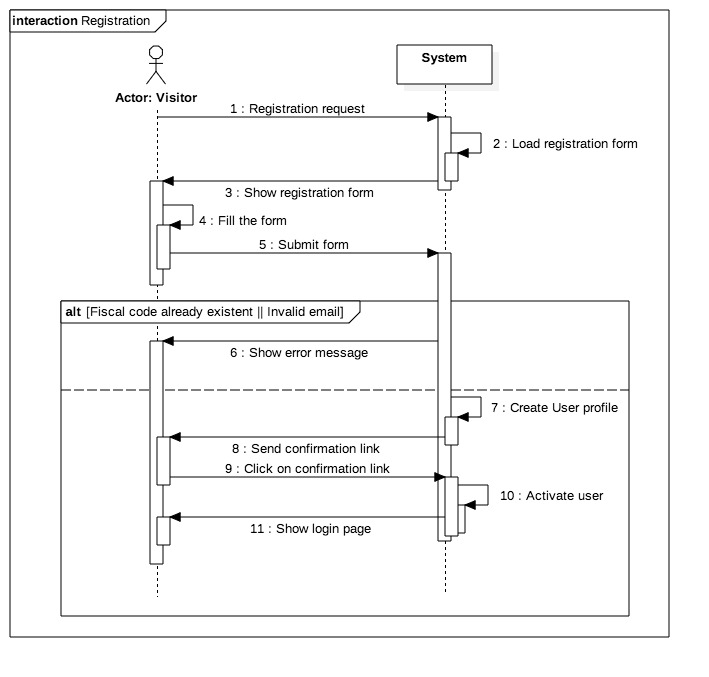
\includegraphics[width=\paperwidth]{./figures/SD_Registration.jpg}}
	\caption{Sequence diagram for the registration}
\end{figure}

\clearpage

\subsection{Login}
\begin{tabular}{lp{8cm}}
	\hline 
	Actors & Visitor  \\ \hline
	Preconditions & The visitor is registered in the system.  \\ \hline
	Execution Flow &  \begin{enumerate}
					\item The Visitor clicks on the login button.
					\item He inserts his email and password.
					\item The system checks inserted data.
					\item The Visitor is redirected to his personal page and becomes an user or a \gls{driver}.
				\end{enumerate}
	 \\ \hline
	 Postconditions & The Visitor is now an user or a \gls{driver} (depends on his keys), he is logged and his capable to use all his reserved functionalities. \\ \hline
	 Exceptions &  The couple of email and login isn't incorrect. The inserted email doesn't refer to any user. In both case the login is refused. \\ \hline
\end{tabular}

\clearpage

\begin{figure}
	\centerline{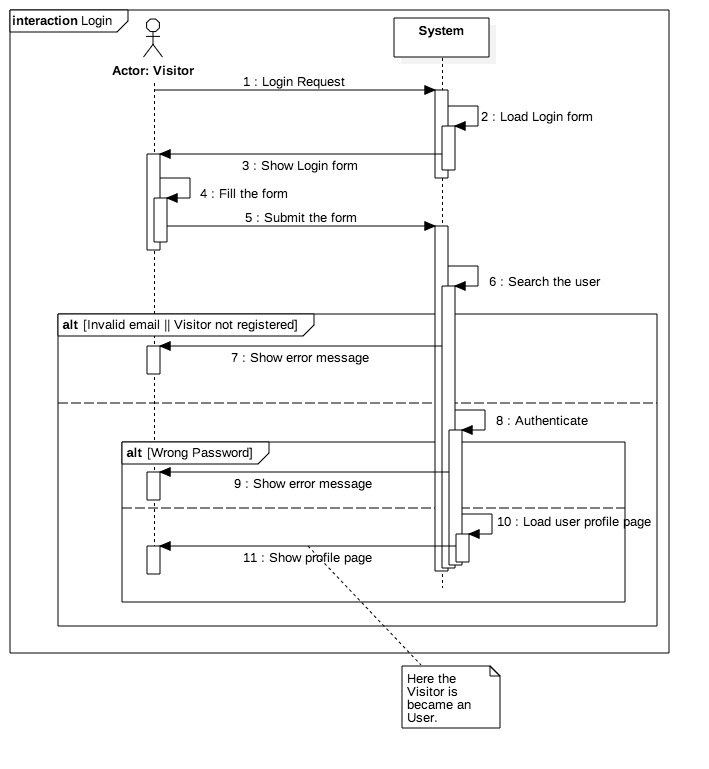
\includegraphics[width=\paperwidth]{./figures/SD_Login.jpg}}
	\caption{Sequence diagram for the login}
\end{figure}

\clearpage

\subsection{Personal Information Management}
\begin{tabular}{lp{8cm}}
	\hline 
	Actors & Users  \\ \hline
	Preconditions & The user is logged into the system.  \\ \hline
	Execution Flow &  \begin{enumerate}
					\item The user selects the related options in his profile page.
					\item The system shows the modification form to the user (name, surname and tax code are not modifiable).
					\item The user modifies the desired information, then submits the form.
					\item The system checks the information and modifies them in the system database. If the email has been modified, the system sends a confirmation link to user.
					\item Only if the user has modified the email, he clicks on the confirmation link to save his new email.
				\end{enumerate}
	 \\ \hline
	 Postconditions & The user's personal information are modified. \\ \hline
	 Exceptions &  A \gls{driver} tries to modify his personal information: the system refuses this operation (only the cab company can handle the \gls{driver}'s data).
The modifications are invalid: the system rejects them.\\ \hline
\end{tabular}

\clearpage

\begin{figure}
	\centerline{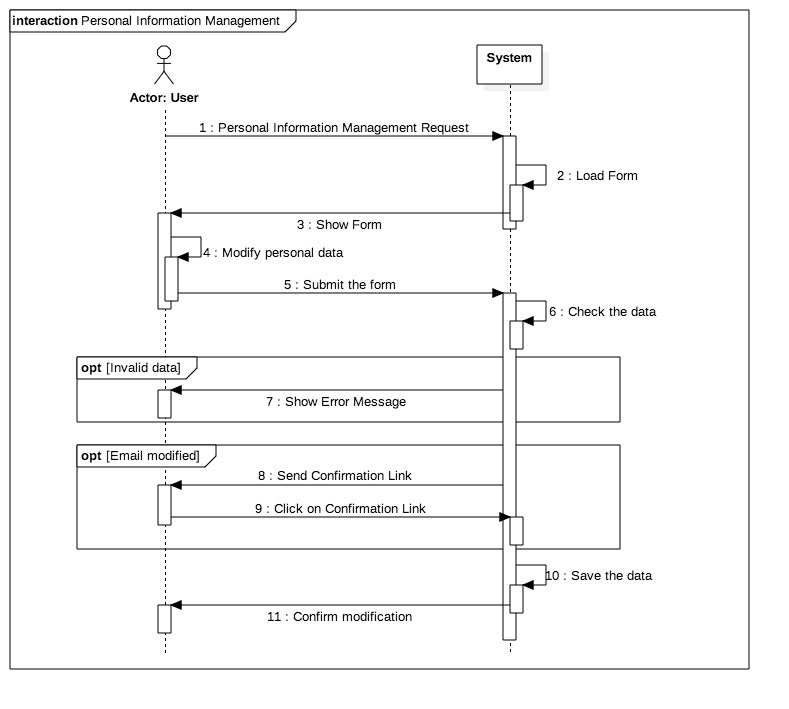
\includegraphics[width=\paperwidth]{./figures/SD_PersonalInformationManagement.jpg}}
	\caption{Sequence diagram for the personal information management}
\end{figure}

\clearpage

\subsection{Zerotime reservation (MA version)}
\begin{tabular}{lp{8cm}}
	\hline 
	Actors & User (or \Gls{driver})  \\ \hline
	Preconditions & The visitor is logged into the system. The driver that will be chosen is into a taxi queue.  \\ \hline
	Execution Flow &  \begin{enumerate}
					\item The user clicks on the related button.
					\item The system calls \gls{gps} system and the latter one calculate the user's position. Then the former one shows a \gls{map} with the position to the user.
					\item The user confirms his position by clicking on the shown popup and then submits the destination by clicking on the \gls{map} or by inserting the address manually.
					\item The system verifies the destination, then confirms it to the user and informs him about travelling time and price.
					\item The ride allocator is involved by the system and it contacts the first driver in the queue. It asks him the availability for the ride. The driver accepts, so the ride allocator ends its work informing the user about the cab carcode, the driver name and the waiting time.
					\item The system saves the ride's information.
				\end{enumerate}
\\ \hline
\end{tabular}
\newpage
\begin{tabular}{lp{8cm}}
	\hline	 
	 %\\ \hline
	 Postconditions & The ride is assigned to the user, a taxi is moving to the position of the user with a driver different from the user. The driver selected for the ride isn't in any taxi queue. The ride is saved on user's history. \\ \hline
	 Exceptions &  The \gls{gps} doesn't work (in this case see the paragraph 3.2.7). The destination is missing: the ride is not sent to the system.\\
	 &
The driver rejects the ride: the system puts him at the end of the queue and contacts the following one. The queue is empty: the system contacts the near areas (special mode).\\
&
The user aborts the ride before system confirmations: the system aborts all operations executed to assign the ride.\\ \hline
\end{tabular}

\subsection{Zerotime reservation (WS version)}
\begin{tabular}{lp{8cm}}
	\hline 
	Actors & User (or \Gls{driver})  \\ \hline
	Preconditions & The visitor is logged into the system. The driver that will be chosen is into a taxi queue.  \\ \hline
	Execution Flow &  \begin{enumerate}
					\item The user clicks on the related button.
					\item The user insert the starting and the destination address directly on the \gls{map} or in the form writing them.
					\item The system checks the correctness of the addresses.
					\item The system confirms the received data to the user and informs him about travelling time and price.
					\item The ride allocator is involved by the system and it contacts the first driver in the queue. It asks him the availability for the ride. The driver accepts, so the ride allocator ends its work informing the user about the cab carcode, the driver name and the waiting time.
					\item The system saves the ride's information.
				\end{enumerate}
\\ \hline
\end{tabular}
\newpage
\begin{tabular}{lp{8cm}}
	\hline	 
	 %\\ \hline
	 Postconditions & The ride is assigned to the user, a taxi is moving to the position of the user with a driver different from the user. The driver selected for the course it isn't in any taxi queue. The ride is saved on user's history. \\ \hline
	 Exceptions &  The destination or the leaving position is missing: the ride is not sent to the system. The inserted data are invalid: the system ignores the request.\\
& The driver rejects the ride: the system puts him at the end of the queue and contacts the following one. The queue is empty: the system contacts the near areas (special mode).\\
& The user aborts the ride before system confirmations: the system aborts all operations executed to assign the ride.
\\ \hline
\end{tabular}
\\
\\
In the following page there is a sequence diagram for both zerotime \gls{reservation} cases.\\

\clearpage

\begin{figure}
	\centerline{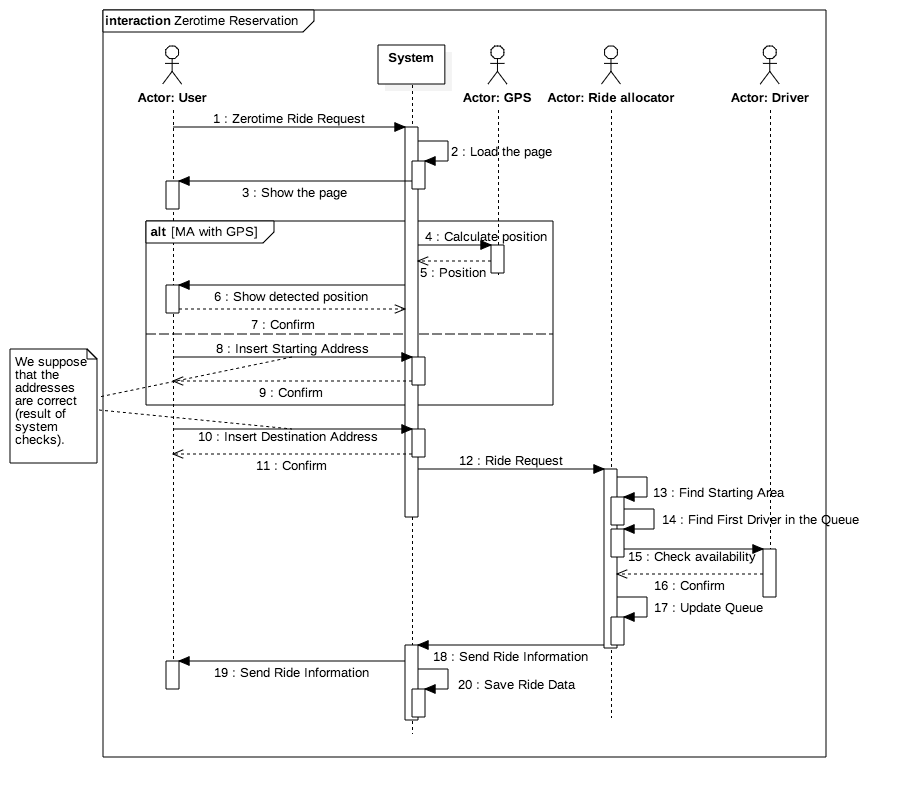
\includegraphics[width=\paperwidth]{./figures/SD_ZerotimeReservation.png}}
	\caption{Sequence diagram for the zero time \gls{reservation}}
\end{figure}

\clearpage

\subsection{Future reservation}
\begin{tabular}{lp{8cm}}
	\hline 
	Actors & User (or \Gls{driver}) \\ \hline
	Preconditions & The visitor is logged into the system. \\ \hline
	Execution Flow &  \begin{enumerate}
					\item The user clicks on \gls{future} \gls{reservation}.
					\item The system shows him a form.
					\item The user fulfills the starting and the destination addresses and the departure time. Afterwards he submits the form.
					\item The system checks the correctness of the received data, then it confirms the data to the user and informs it about travelling time and price.
					\item The system saves the ride's information.
					\end{enumerate}
	 \\ \hline
	 Postconditions & The ride is saved on user's history and it is saved on the system. The system is able to perform the ride request ten minutes before the departure time.\\ \hline
	 Exceptions & The destination or the starting position or the departure time is missing: the ride is not sent to the system.\\
				& The starting or the destination address is invalid. The departure time is not between 1 hour and 30 days from the current time. In both cases the system rejects the ride.  \\ \hline
\end{tabular}\\

\begin{figure}
	\centerline{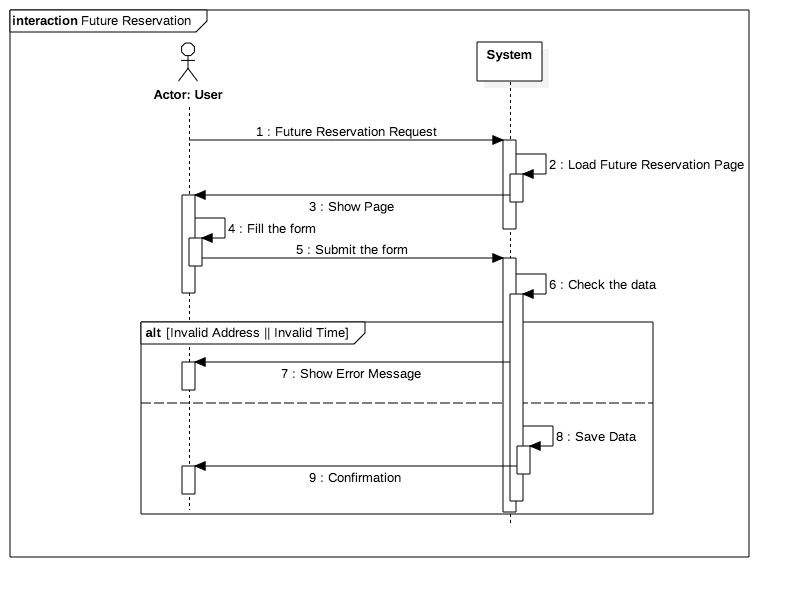
\includegraphics[width=\paperwidth]{./figures/SD_FutureReservation.jpg}}
	\caption{Sequence diagram for the \gls{future} \gls{reservation}}
\end{figure}

\subsection{Start waiting time}
\begin{footnotesize}
	Note: every time a driver ends a ride, he has to use this functionality.
\end{footnotesize}\\
\begin{tabular}{lp{8cm}}
	\hline 
	Actors & \Gls{driver}  \\ \hline
	Preconditions & The driver is logged in the system. The driver is into his working hours, thus he has inserted a work shift that contains the current time. [If he is notifying the system that he is no longer available the driver is inserted in the queue related to his current position.] \\ \hline
	Execution Flow &  \begin{enumerate}
					\item The driver clicks the start waiting time button.
					\item The system shows him a \gls{map} and an input field for address.
					\item The driver can click on a \gls{map} area (the \gls{map} was previously splitted in all the city areas and has a default selection on the position detected by \gls{gps}) or insert manually his address.
					\item The system involves the ride allocator. The latter one adds [remove] the driver to the queue of driver's current area. Then the ride allocator informs the system about the result of the operations.
					\item The system saves the data received by the ride allocator and confirms the operation to the driver. Only when the driver is added to a queue an additional information is given: the number of drivers before him.
				\end{enumerate}
	 \\ \hline
	 Postconditions & The driver is put in the tail [put off] of the queue of the area where he is.\\
	 				& The driver isn't put in any other queue. \\ \hline
	 Exceptions &  The \gls{gps} doesn't work: the system gives the driver the possibility of manually insert his address (and links it with the related area). \\ \hline
\end{tabular}

\begin{figure}[h!]
	\centerline{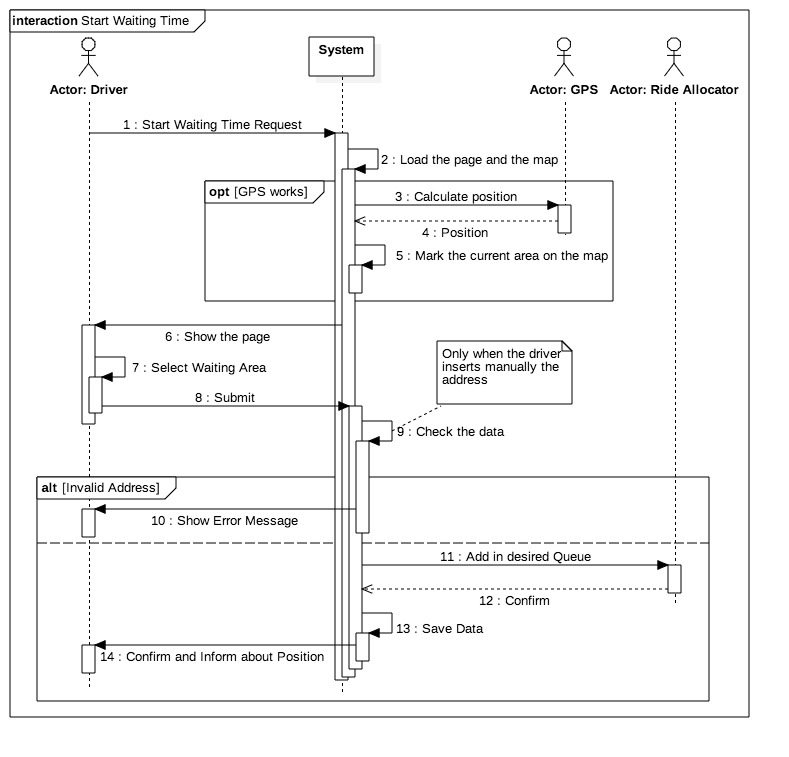
\includegraphics[width=\paperwidth]{./figures/SD_StartWaitingTime.jpg}}
	\caption{Sequence diagram for the start waiting time function. The case of not availability is not represented in this diagram, but the only change is on message 11. (Remove from the current Queue)}
\end{figure}

\clearpage

\subsection{Work shifts management}
\begin{tabular}{lp{8cm}}
	\hline 
	Actors & \Gls{driver}\\ \hline
	Preconditions & The driver is logged in the system.\\ \hline
	Execution Flow &  \begin{enumerate}
					\item The driver clicks on work shifts management button.
					\item The system shows him the current month table (the rows represents the hours, the columns the days) where are visible all previous inserted shifts.
					\item The driver fills the desired work hours by clicking on the cells, then submits the forms.
					\item The system validates the data and notifies it the user.
					\end{enumerate}
	 \\ \hline
	 Postconditions & The new shifts are saved in the system according to the laws and the work contract of the driver (e.g. maximum daily hours, number of work hours in a month and so on). No shifts are overlapped.\\ \hline
	 Exceptions & The driver inserts less hour than the minimum requested in a month: the system accepts the new shifts and notifies to driver that he has to insert more shifts. The driver insert illegal shifts (opposed to the laws or opposed to cab company rules or overlapped): the system refused them and notifies the driver.  \\ \hline
\end{tabular}

\begin{figure}
	\centerline{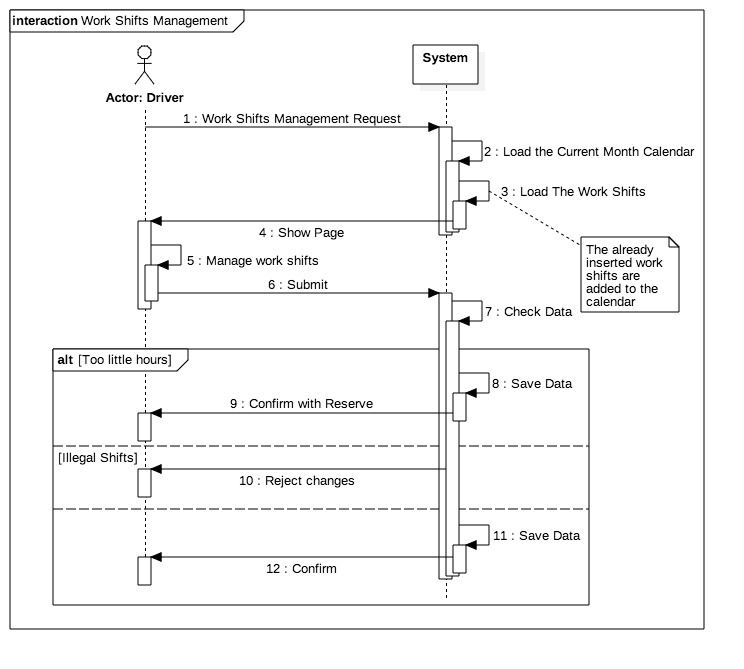
\includegraphics[width=\paperwidth]{./figures/SD_WorkShiftsManagement.jpg}}
	\caption{Sequence diagram for the work shifts management}
\end{figure}

\subsection{Check the reservations}
\begin{tabular}{lp{8cm}}
	\hline 
	Actors & User \\ \hline
	Preconditions & The user is logged in the system.
All the historical (already done) and the zerotime \glspl{reservation} can be showed only. \\ \hline
	Execution Flow & \begin{enumerate}
					\item The user clicks on the Check \glspl{reservation} button.			
					\item The system shows the user all historical, zerotime and \gls{future} \glspl{reservation} in descending order by date. In particular, for the latter ones the system allows to modify or cancel them by a button.
					\item If the user wants to modify a \gls{reservation} he clicks on related button and system redirects him to the \gls{future} booking page (already filled in all boxes with current data).
					\item If the user wants to cancel a booking he clicks on related button. Then the system shows him a confirmation message.
				\end{enumerate}
	 \\ \hline
	 Postconditions & All the historical (or zerotime) \glspl{reservation} are saved again without changes. All \gls{future} \glspl{reservation} are still in the system unless they are cancelled or modified by user. In the other cases the \gls{reservation} are correctly modified or deleted.\\ \hline
	 Exceptions & The user tries to modify or cancel a \gls{future} \gls{reservation} less that 15 minutes before the departure time: the system rejects the operation and informs the user.  \\ \hline
\end{tabular}

\clearpage

\begin{figure}
	\centerline{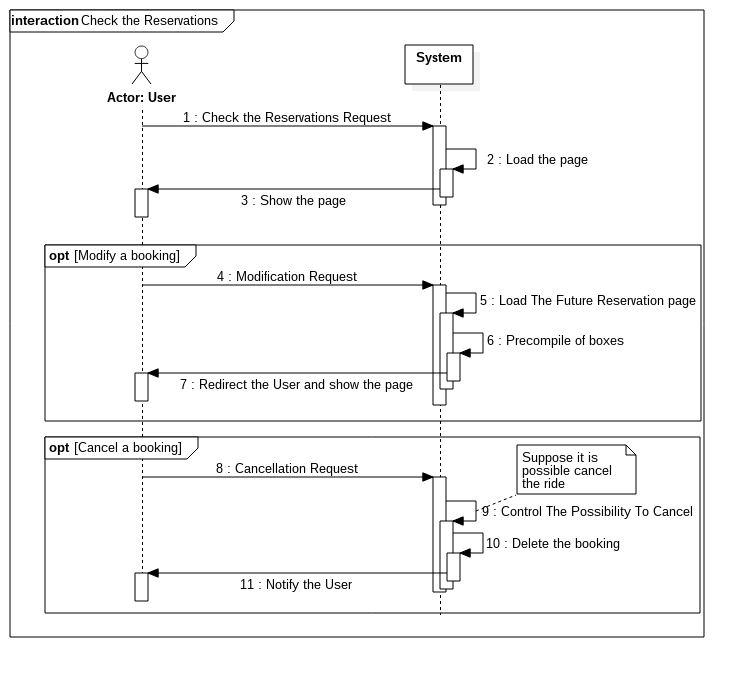
\includegraphics[width=\paperwidth]{./figures/SD_CheckReservations.png}}
	\caption{Sequence diagram for the check \glspl{reservation} function}
\end{figure}

\clearpage

\subsection{Read the alerts}
\begin{tabular}{lp{8cm}}
	\hline 
	Actors & User \\ \hline
	Preconditions & The user is logged in the system.  \\ \hline
	Execution Flow &  \begin{enumerate}
						\item The User clicks on Read the \glspl{alert} button.
						\item The system shows the user all his \glspl{alert} in descending date order.
					\end{enumerate}
	 \\ \hline
	 Postconditions & The \glspl{alert} are not changed or removed by the system. \\ \hline
	 Exceptions & None.  \\ \hline
\end{tabular}\\
\\

\begin{figure}[h!]
	\centerline{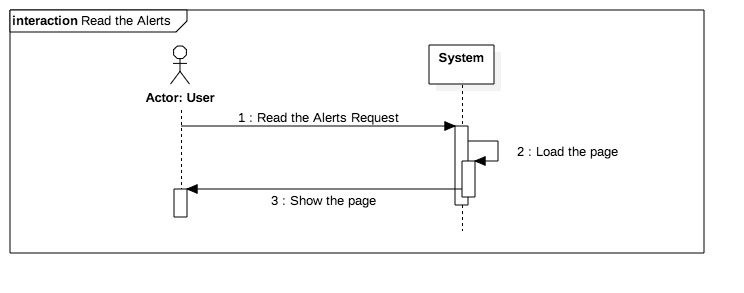
\includegraphics[width=\paperwidth]{./figures/SD_ReadTheAlerts.jpg}}
	\caption{Sequence diagram for the read the \glspl{alert} function}
\end{figure}



\clearpage

\section{Entities Behaviour}
In this section the behaviour of some entities presented in \figurename~\ref{cDia} is exposed using UML state chart diagrams.
\subsection{Zerotime Ride Class}
\begin{figure}[h!]
	\centerline{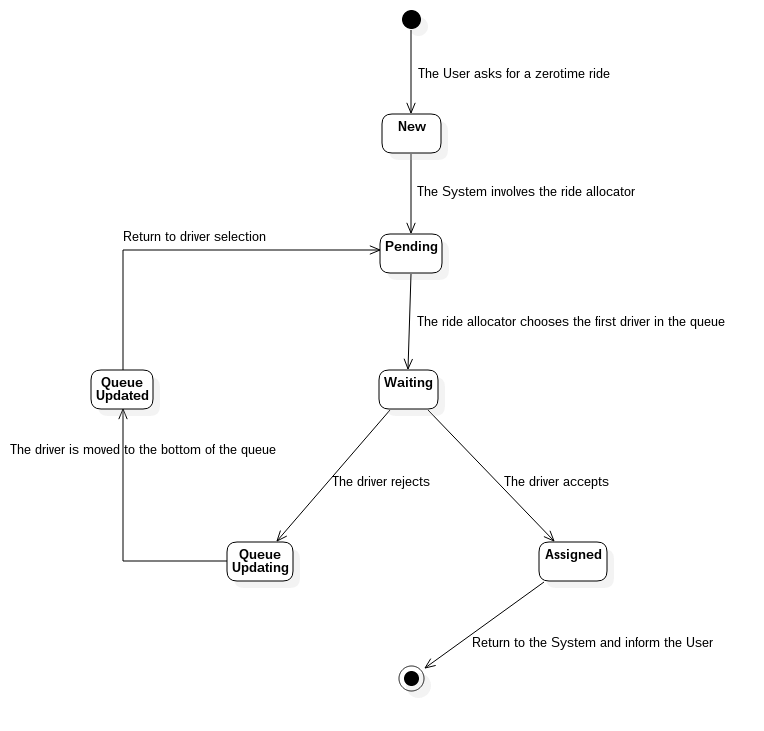
\includegraphics[width=\textwidth]{./figures/Statechart_ZerotimeRideClass.png}}
	\caption{The behaviour of the Zerotime ride class presented via UML state diagram}
\end{figure}

\clearpage
\subsection{Future Ride Class}
\begin{figure}[h!]
	\centerline{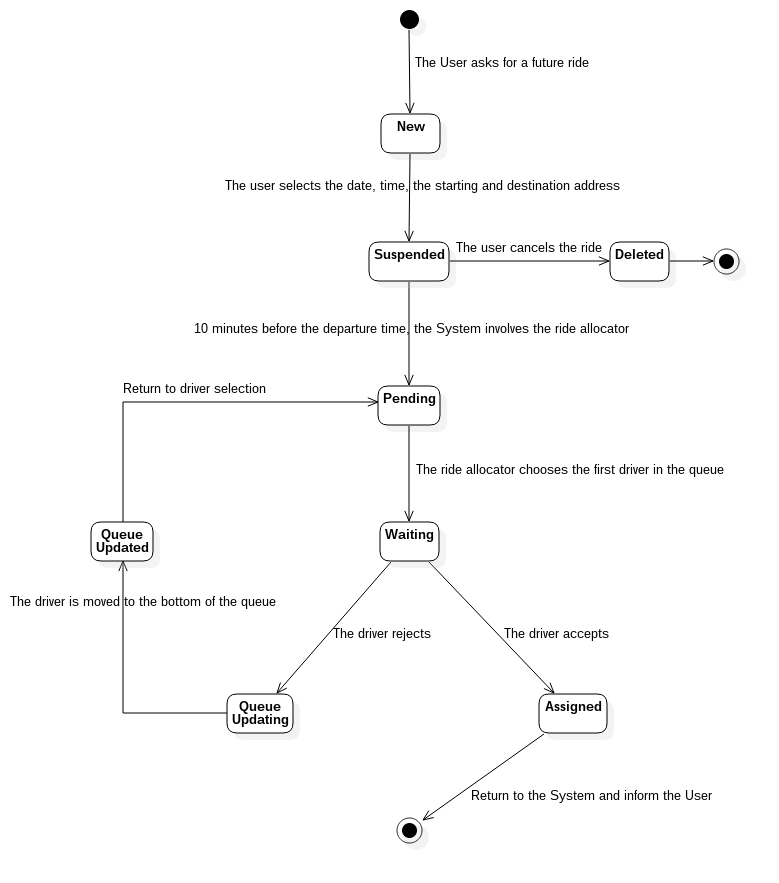
\includegraphics[width=\textwidth]{./figures/Statechart_FutureRideClass.png}}
	\caption{The behaviour of the \Gls{future} ride class presented via UML state diagram}
\end{figure}

\acresetall